\section{Ablauf chemischer Reaktionen}

\subsection{Freiwlligkeit der Reaktionen}

\subsubsection{Enthalpie H / Reaktionsenthalpie $\Delta H_R$}
Prinzip Energieminimum: Stoff will energiearmen Zustand erreichen!\\
$\Delta H_R = H_{Produkte} - H_{Edukte} \quad [H] = \frac{kJ}{mol * K}$\\

\subsubsection{Entropie S / Reaktionsentropie $\Delta S$}
Prinzip Energiemax: Stoffe eines Sys. mögl. grosse unordnung an!\\
\begin{tabular}{p{5.5cm}l}
$\Delta S = \sum S^0_{Produkte} - \sum S^0_{Edukte}$ & $[\Delta S] = \frac{\color{red}J}{mol * K}$
\end{tabular}\\
$S^0$: Molare Standartentropie (1mol des Stoffs bei Std.Bedingungen)
\subsubsection{Freie Enthalpie $\Delta G$}
Beschreibt Freiwilligkeit der Reaktion:\\
\begin{tabular}{p{5.5cm}l}
$\Delta G = \Delta H - T * \Delta S$ & $[\Delta G] = \frac{kJ}{mol}$
\end{tabular}
\begin{itemize}
    \item $\Delta G < 0:$ Exergon (freiwillige Reaktion)
    \item $\Delta G > 0:$ Endergon(Unfreiwillige Reaktion)
\end{itemize}

\subsubsection{Aktivierungsenergie/Reaktionsgeschw./Katalysatoren}
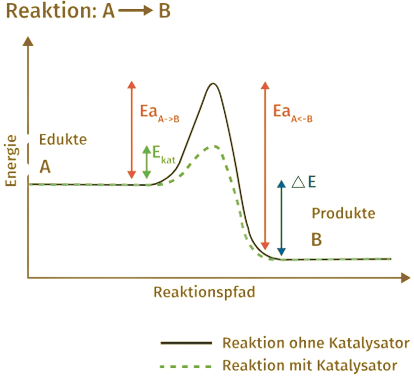
\includegraphics[height=4cm]{pictures/Katalysator.png}\\
RGT-Regel: $\Delta$ T von 10 = verdoppelung der RG!\\
Katalysator = Stoff welcher an reakt. Teilnimmt, jedoch nicht verbraucht wird.\\
Beschleunigt Reaktion: $E_{AKat} \ll E_{ANorm}$\\
$\Delta$ G sowie $\Delta H_R$ bleiben gleich!\\
Sind selektiv (wirken nicht mit allen stoffen)
